\chapter{Introduction}
\section{Motivation}
As human beings, we visually perceive and experience our whole world in terms of colors, resulting from various physical phenomina involving interaction between light and matter. Particularly in nature, there are basically two main causes for color production. Firstly, due to pigmentation, which occurs since certain molecules in a biological structure selectively absorb or reflect specific wavelengths from an incident light source. And secondly because of structural colors which are the result of physical interaction of light with a nanostructure, exclusively relying on the structuring of the material and not any other property. A natural diffraction grating is a semitransparent layer of biological nano-structures which exhibits a certain degree of regularity to produce structural colors by diffracting an incident light source. One particular example for such biological color production are the colors we can see when having a closer look at the illuminated skin of snakes, as shown in figure $\ref{fig:snakespecies}$.

\begin{figure}[H]
  \centering
  \subfigure[Xenopeltis snake]{
    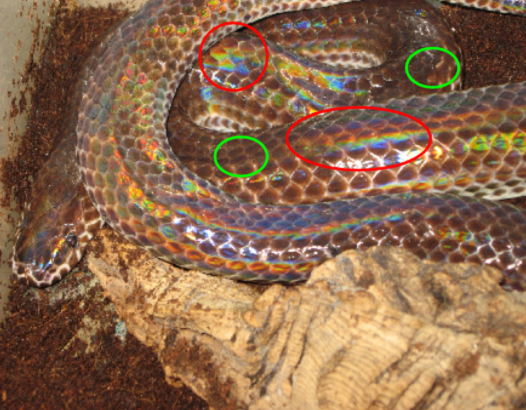
\includegraphics[scale=0.39]{background/xenopeltissnake.png}
    \label{fig:xenospeicies}
  }
~
  \subfigure[Elaphe Guttata snake]{
    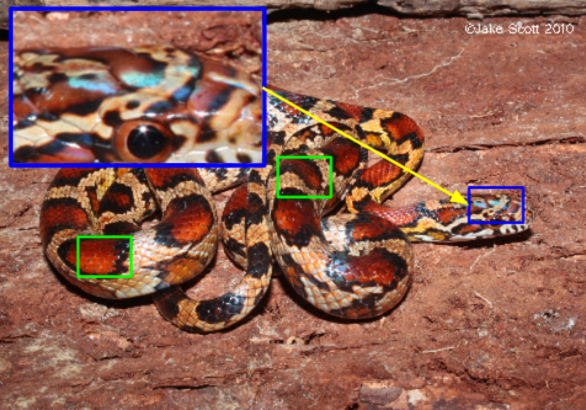
\includegraphics[scale=0.39]{background/elaphesnake.png}
    \label{fig:elpahespecies}
  }
  \caption[Example of Biological Color Production]{Examples of pigmentation color (green circles) and structural color (red circles) on different snake species$\footnotemark$.}
  \label{fig:snakespecies}
\end{figure}
\footnotetext{image source of figure $\ref{fig:xenospeicies}$ \texttt{http://www.snakes-alive.co.uk/gallery\textunderscore 5.html} and figure $\ref{fig:elpahespecies}$ \texttt{http://www.the-livingrainforest.co.uk/living/view\textunderscore price.php?id=464}} 

Some species like Xenopeltis express structural colors in form of iridescent patterns along their scales way strongerthan others like Elaphe species. The reason for this lies on the nanostructure of their skins. There are a vast amount of additional reasons for producing structural colors in nature, such as thin film interference, intra-cellular photonic crystals or diffraction gratings. More detailed examples are shown in figure $\ref{fig:structuralcolorexamples}$. 

\begin{figure}[H]
  \centering
  \subfigure[Thin Film Interference soap bubble]{
    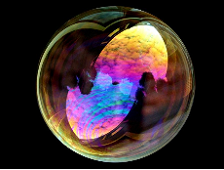
\includegraphics[scale=0.6]{background/soapbubble.png}
    \label{fig:soapbubble}
  }
~
  \subfigure[Multilayer Interference on abdomen of beetle]{
    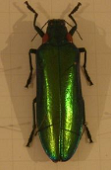
\includegraphics[scale=0.6]{background/beetle.png}
    \label{fig:beetle}
  }
~
  \subfigure[Photonic crystals in Wings of butterfly]{
    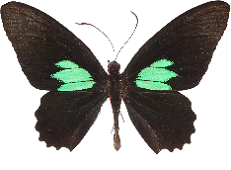
\includegraphics[scale=0.6]{background/butterflypc.png}
    \label{fig:butterflyphotoniccristals}
  }

  \subfigure[Scattering of light on butterfly wing]{
    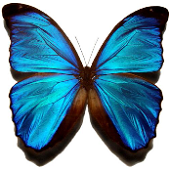
\includegraphics[scale=0.6]{background/butterflyscattering.png}
    \label{fig:butterflyscattering}
  }
~
  \subfigure[Artificial Diffraction Grating on CD]{
    
\includegraphics[scale=0.6]{background/cd.png}
    \label{fig:cddiffractiongrating}
  } 
~
  \subfigure[Natural Diffraction Grating on snake skin]{
    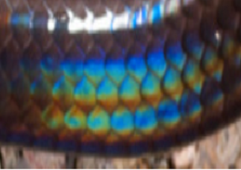
\includegraphics[scale=0.6]{background/snakeskin.png}
    \label{fig:snakediffractiongrating}
  }   
  
  \caption[Structural color examples]{Examples$\footnotemark$ for structural colors on the wings and the abdomen of insects, liquids, synthetic structures, and on scales on the skin of reptiles.}
  \label{fig:structuralcolorexamples}
\end{figure}
\footnotetext{image source of figure:
\begin{itemize}
  \item \ref{fig:soapbubble}: \texttt{http://www.ualberta.ca/\textasciitilde pogosyan/teaching/PHYS\textunderscore 130/FALL\textunderscore 2010/lectures/lect33/lecture33.html}
  \item \ref{fig:beetle}: \texttt{http://www.itp.uni-hannover.de/\textasciitilde zawischa/ITP/multibeam.html}
  \item \ref{fig:butterflyphotoniccristals}: \texttt{http://upload.wikimedia.org/wikipedia/commons/a/a4/Parides\textunderscore sesostris\textunderscore MHNT\textunderscore dos.jpg}
  \item \ref{fig:butterflyscattering}: From paper \cite{struccolor}, figure 6.
  \item \ref{fig:cddiffractiongrating}: \texttt{http://cnx.org/content/m42496/latest/?collection=col11428/latest}
  \item \ref{fig:snakediffractiongrating}: \texttt{http://www.snakes-alive.co.uk/gallery\textunderscore 5.html}
  \end{itemize}
}

As far back as in the 17th century, Robert Hooke was able to relate the cause of structural colors to the the microstructure of a material. During his examinations of peacock feathers he found that the colors could be made disappear by wetting the feathers and further observed that the feathers are made of tiny ridges. Building on top of the latest knowledge about interference, Newton related structural colors with wave interference. Recently, in the field of computer graphics, many researchers have developed models to render structural colors, but most of the currently available models are not able to perform interactive rendering or are oversimplified and thus cannot model accurately the effect of diffraction. \\

This thesis investigates this particular problem in detail and provides a solution for rendering structural colors due to diffraction on natural gratings.

\section{Goals}
The purpose of this thesis is firstly, to simulate physically accurate structural colors caused by the effect of diffraction on various biological structures and secondly implement this simulation as a renderer with interactive behaviour. We mainly focus on structural colors generated by natural diffraction gratings. In particular the approach presented in this thesis applies to surfaces with quasiperiodic structures at the nanometer scale which can be represented as height fields stored in gray-scale images. \\

Natural gratings like this are found on the scale of reptiles, wings of butterflies or the bodies of various insects but we restrict ourself and focus on snake skins. The data of our discrete valued height fields, which are representing the surface of a measured snake skin was acquired using atomic force microscopy (AFM)$\footnote{All data is provided by the Laboratory of Artificial and Natural Evolition in Geneva. See their website:\texttt{www.lanevol.org}}$. Figure $\ref{fig:xenopeltisafm}$ shows a measured height field of a Xenopeltis snake, which stored in a grayscale image. The surface of its skin is composed of many finger like structures. Locally, these fingers seem to be very regularly aligned (red box). However, globally, we observe that the alignment of the fingers is irregularly curved (indicated by green curves) along the whole surface. This kind of global irregularity is why it makes it hard to model the structural complexity of natural gratings$\footnote{E.g. by relying on statistical methods, caputuring surface details by introducing an appropriate distribution function of the finger strucures.}$.

\begin{figure}[H]
  \centering
  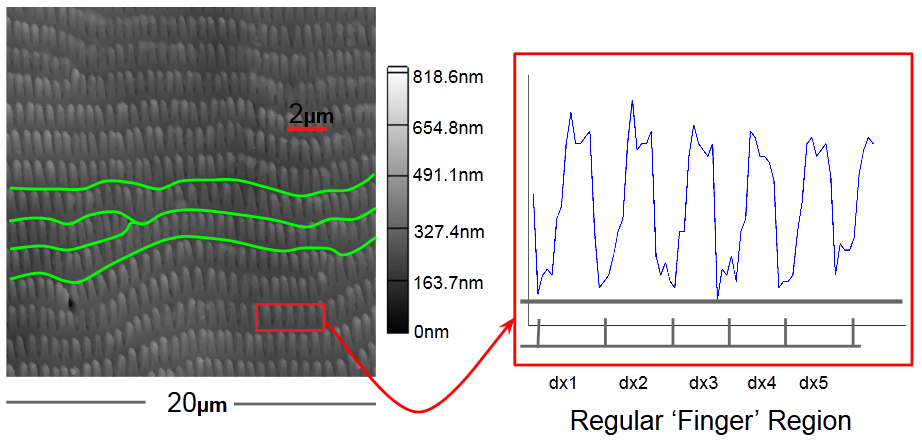
\includegraphics[scale=0.5]{background/samplenaturalgrating.png}
  \caption[Xenopeltis AFM image]{Height field of a Xenopeltis snake$\footnotemark$ skin taken by AFM and stored as a grayscale image. 
  Locally, this natural grating consists of regularly aligned (red box) finger-like substructures, but globall we observe a curved alignment of these structures (green curves).}
  \label{fig:xenopeltisafm}
\end{figure}
\footnotetext{This image was provided by the LANE lab in Geneva}

The renderer discussed in this thesis is based on the pioneering work of J. Stam about diffraction shaders $\cite{diffstam}$ in which he formulated a BRDF modelling the effect of diffraction. Nevertheless we have to adapt his BRDF model since his model assumes, that a given surface of a grating can either be formulated by an analytical function, and therefore has a closed form solution or it is simple enough to be modelled effectively by relying on statistical methods. However, we are dealing with natural diffraction gratings, represented as explicitly formulated height fields, which unfortunately are neither known analytically nor do they fit into simple statistical models. This thesis thus proposes an extension of J. Stam's work for the complex case of explicitly defined, discrete and quasi-periodic height field structures. \\

In the following section a breif overview of previous work relevant and related to this work will be presented.

\section{Previous work}
The first scientific descriptions of structural colors was previousely by Hooke in 1665 in his book Micrographia$\cite{hookemicro}$. Hooke investigated feathers of peacocks using one of the first microscopes from his time and found out that the colors on the feather were canceled out whenever a drop of water moistened the feather. He proposed the speculation that a layer of thin plates and air were responsible for reflecting the light and thus he related the structure of the feather to colors. In Newton's book Opticks$\cite{newtonopticks}$ he described that the colors of the peacock feather are related to the thinness of the transparent part of the feathers. Around 1800 T.Young explains structural colors as a result of wave interference using his double-slit experiment$\footnote{See \texttt{http://en.wikipedia.org/wiki/Double-slit\textunderscore experiment}}$$\cite{doublslit}$, published in the journal Philosophical Transactions of the Royal Society. \\

In the field of computer graphics, J.Stam$\cite{diffstam}$ was the first one who was able to develop reflection models based on wave optics capturing the effect of diffraction due to nano-structure height fields. His model is an approximation of far field diffraction$\footnote{See \texttt{http://en.wikipedia.org/wiki/Fraunhofer\textunderscore diffraction}}$ effects relying on the Kirchhof integral$\footnote{See \texttt{http://en.wikipedia.org/wiki/Kirchhoff\textunderscore integral\textunderscore theorem}}$. For a certain class of surfaces which can be modelled as a height field he provides an analytical solution of the BRDF model. He assumes homogeneity of the structure and then the main idea of his model is the formulate a BRDF as the Fourier Transform applied on the the correlation function of the given height field. However, the height fields that Stam is dealing with are either extremely regular or can be considered as a superposition of randomly distributed bumps forming a periodic like structure relying on probabilistic distribution theory$\footnote{See \texttt{http://en.wikipedia.org/wiki/Probability\textunderscore distribution}}$. Both height field assumptions allow him to derive an analytical solution using statistical models. However, the height field we are dealing with are measured, complex, biological nano-structures and thus they do not exhibit regularity at a global scale as demonstrated in figure $\ref{fig:xenopeltisafm}$. It is not sufficient to superimpose one particular nano finger (considering it as a bump) for capturing the complexity of the measured structure since this poses a non-trivial problem of modeling the distribution of nano finger statistically. Therefore, we cannot directly use Stam's BRDF model when we want to perform interactive rendering for diffraction effects of natural gratings.\\

In 2012 Cuypers et all $\cite{reflectancediffmodel}$ proposed a wave based Bidirectional scattering distribution function (BSDF$\footnote{See \texttt{http://en.wikipedia.org/wiki/Bidirectional\textunderscore scattering\textunderscore distribution\textunderscore function}}$) denoted as WBSDF.
Using the rendering equation and Wigner Distribition Functions$\footnote{See \texttt{http://en.wikipedia.org/wiki/Wigner\textunderscore distribution\textunderscore function}}$ (WDF) they related their WBSDF model to the incoming wavefront and hence, their model can be adapted such that it can be rendered by a Monte Carlo renderer. The advantage of their model over Stam's is that their models also captures near field diffraction effects. A disadvantage their model is computational expensive since the WDF of a two dimensional surface is a four dimensional function and therefore can hardly be used in order to perform interactive rendering. \\

Linday and Agu $\cite{reflectancediffmodel}$ proposed an approach in order to perform interactive rendering diffraction effect by precomputing and storing their BRDF model using spherical harmonics. Nonetheless, for complex natural gratings their BRDF may be insufficient accurate since their approach is using low order spherical harmonics.

\section{Thesis Structure}
The reminder of this thesis is organised as follows: Due to the fact that this thesis has a rather advanced mathematical complexity, chapter 2 introduces some important definitions about modelling light in computer graphics and some wave theory. These concept are required in order to be able to follow our later derivations. This is followed by a brief summary of J. Stam's Paper about diffraction shaders, since his BRDF formulation is the basis of our derivations. \\

In chapter 3 we adapt Stam's BRDF model step-wise in a way that we will end up with a representation which can be implemented as an interactive diffraction renderer when using natural diffraction gratings. We also propose an alternative formulation, the so called PQ approach in this chapter and discuss its short-comings. \\

Chapter 4 addresses the practical part of this thesis, the implementation of our diffraction model, explaining all precomputation steps and how rendering is preformed in our reference framework for this thesis. \\

Chapter 5 gives some further insight about diffraction by explaining the topic about diffraction grating in depth. Furthermore, within this chapter we evaluate the qualitative validity of our BRDF model applied on different surface gratings by computing their reflectance and comparing the results to the grating equation under similar conditions. \\

Chapter 6 presents our rendered results, first the so called BRDF maps for all our gratings and shading approaches under various shading parameters and then the actual renderings on a snake skin. And finally chapter 7 contains the conclusion of this thesis discussing what has been achieved in this thesis and all the drawbacks of the proposed method. It also contains a note about some of my personal experiences during this thesis.
